%%%%%%%%%%%%%%%%%%%%%%%%%%%%%%%%%%%%%%%%%%%%%%%%%%%%%%%%%%%%%%%%%%%%%%%%%%%%%%%%
%2345678901234567890123456789012345678901234567890123456789012345678901234567890
%        1         2         3         4         5         6         7         8


%\documentclass[twocolumn,journal]{IEEEtran}
\documentclass[twocolumn,journal]{IEEEtran}
%\documentclass[letterpaper, 10 pt, conference]{ieeeconf}  % Comment t                                                      his line out
                                                          % if you need a4paper
%\documentclass[a4paper, 10pt, conference]{ieeeconf}      % Use this line for a4
                                                          % paper

\IEEEoverridecommandlockouts                           % This command is only
                                                          % needed if you want to
                                                          % use the \thanks command
\overrideIEEEmargins
% See the \addtolength command later in the file to balance the column lengths
% on the last page of the document

\newtheorem{theorem}{Theorem}
\newtheorem{definition}{Definition}
\newtheorem{corollary}{Corollary}
\newtheorem{example}{Example}
\newtheorem{assumption}{Assumption}
\newtheorem{hypothesis}{Hypothesis}
\newtheorem{lemma}{Lemma}
\newtheorem{remark}{Remark}
\newtheorem{notation}{Notation}
\newtheorem{algorithm}{Algorithm}
%\newcommand{\for}{\textbf{for}}
%\newcommand{\STATE}{\quad}

% The following packages can be found on http:\\www.ctan.org
\usepackage{graphics} % for pdf, bitmapped graphics files
\usepackage{epsfig} % for postscript graphics files
\usepackage{mathptmx} % assumes new font selection scheme installed
\usepackage{times} % assumes new font selection scheme installed
\usepackage{amsmath} % assumes amsmath package installed
\usepackage{amssymb}  % assumes amsmath package installed
\usepackage{algorithm}
\usepackage{algorithmic}
\usepackage{multirow}
\usepackage{amsmath}
\usepackage{xcolor}

\title{\LARGE \bf
The Equivalence issue of two kinds of controller of Boolean control network}

%\author{Jianquan Lu$^*$, J\"{u}rgen K urths, Jinde Cao, \IEEEmembership{}
\author{Meilin li, Jianquan Lu \IEEEmembership{Member,~IEEE}

\thanks{ Meilin Li is is with the Department of Mathematics, Southeast
University, Nanjing 210096, China {\tt\small 220151318@seu.edu.cn}}
\thanks{Jianquan Lu is with the Department of Mathematics, Southeast University, Nanjing 210096, China
{\tt\small jqluma@seu.edu.cn}}%
\thanks{ {\tt\small }}
\thanks{}
\thanks{}
\thanks{} }
\begin{document}

\maketitle
\thispagestyle{empty}
\pagestyle{empty}


%%%%%%%%%%%%%%%%%%%%%%%%%%%%%%%%%%%%%%%%%%%%%%%%%%%%%%%%%%%%%%%%%%%%%%%%%%%%%%%%
\begin{abstract}
In this paper, the equivalence issue between state feedback controller and free control sequence in Boolean control network is investigated. Based on the algebraic representation of logical equation of semi-tensor product of matrices (STP), we proof that a Boolean control network can be stabilized to a cycle or a point via free control sequence if and only if there is a state feedback controller which can drive the Boolean control network stabilized to the cycle or the point. Then, two algorithms are provided to find the state feedback controller. After that, we prove that if a BCN is global controllable by free control sequence, the BCN is not necessarily global controllable by the state feedback controller. At last, a example is given to illustrate the results in this paper.
\end{abstract}


\begin{keywords}
Boolean control network, STP, free control sequence, state feedback controller.
\end{keywords}
%%%%%%%%%%%%%%%%%%%%%%%%%%%%%%%%%%%%%%%%%%%%%%%%%%%%%%%%%%%%%%%%%%%%%%%%%%%%%%%%
\section{INTRODUCTION}
With the development of system biology, the study of Boolean network (BN) has aroused widespread attention in many different areas. The BN was proposed by Kauffman \cite{Fox1993Review} for modeling genetic regulatory network, and it becomes a powerful tool to analyzing cellular networks. In recent years, the BN has been extensively investigated in many fields \cite{Huang2000Shape}\cite{Kauffman1989The}\cite{Stefan2011Robustness}\cite{Stern1999Emergence}. BN provides a good theoretical framework to analysis the properties of system. One of the purposes of BN modeling is used to propose a method to find control strategies for complex biological systems. The BN with inputs called Boolean control network (BCN), naturally, the control inputs only take one of two values 1 and 0: value 1 indicates that at this time point, the particular interference is being active, and value 0 indicate at this time point the interference is stopped.

Recently, a new matrix product named semi-tensor product (STP) of matrix was proposed by Cheng and his co-workers \cite{Cheng2003On}. STP generalizes the conventional product of matrix, any two matrices can multiply by using STP. Using STP, we can convert a logic equation into an algebraic equation, then BN can be expressed as linear discrete time system \cite{Cheng2003On}. The use of STP provides a efficient mathematical tool for many problems of BN and BCN. There are many studies about BN and BCN based on STP. In \cite{Fornasini2013Observability}, the author proposed a method to reconstruct the BCN based on STP. In \cite{Laschov2012Controllability}, a necessary and sufficient condition for controllability of BCN was proposed in different structure matrix. There are many results about controllability and observability of BCN, see  \cite{Akutsu2007Control}\cite{Langmead2009Symbolic}\cite{Meng2015Controllability}\cite{Li2011Controllability}\cite{Cheng2011Realization}.

The stabilization problem is one of the basic issues of BCN which have been studied in recent years by using STP \cite{Cheng2011Stability}. In \cite{Cheng2011Stability}, the author investigate the stabilization of BCN with free control sequence, which means that the inputs are not related to time and states changing freely. In some cases, the system may need to stabilized to a subset of state space, instead of to a single point. The set stabilization of BCN studied in \cite{Guo2015Set}, Guo \textit{et al.} provide a necessary and sufficient conditions for set stabilizability and set stability based on the invariant subsets. In \cite{Rui2013State}, Li \textit{et al.} proposed a feedback control design approach to achieve stabilization of BCN.

Motivated by state feedback control and free control sequences in stabilization of BCN, we guess whether these two control approaches in stabilization of BCN are equivalent. So in this paper, the equivalence problem of state feedback control and free control sequences in stabilization of BCN is investigated. First, we prove the equivalence between state feedback controller and free control sequences in stabilization of BCN. Second, a algorithm is proposed to obtain a state feedback controller if the system can be stabilized by free control sequences. Then we give a example to illustrate that if a BCN is controllable by free control sequence there not necessarily exist a state feedback controller, and we give a existence condition of the state feedback controller if the BCN is controllable by free control sequence.

The remainder of this paper is organized as follows. Section 2 gives some preliminary results about STP and the problem formulation. Section 3 present our results about equivalence between state feedback controller and free control sequences in stabilization of BCN. An example illustrate the results obtained in this paper in Section 4. At last, there is a conclusion about this paper.



\section{Preliminaries}
In this section, the STP of matrices is firstly reviewed. Then some preliminary results about STP are revisit. At last, we propose the problem formulation.

\begin{definition}\label{STP}
Let$A\in\mathbb{R}^{n\times m}$, $B\in \mathbb{R}^{p\times q}$. The $semi-tensor$ $product$ of $A$ and $B$ is
\begin{equation}
A\ltimes B=(A\otimes I_{\frac{l}{m})}(B\otimes I_{\frac{l}{p}})
\end{equation}
where $l$ is the least common multiple of $m$ and $p$.
\end{definition}

In definition \ref{STP}, if $m=p$, then the STP of $A$ and $B$ is reduced to their conventional matrix product $AB$.
We identify $\Delta_{2}\sim \mathcal{D}$ i.e $(\delta^1_2\sim 1,\delta^2_2\sim 0)$, and $\delta^1_2(\delta^2_2)$ is called the vector form of logical value $1(0)$.

\begin{lemma}\label{lemma}\cite{Cheng2011Analysis}
Any Boolean function $f(x_1,x_2,...,x_n)$ with variables $x_1,x_2,...,x_n\in \Delta_2$ can be expressed as a multi-linear form:
\begin{equation}
f(x_1,x_2,...,x_n)=Fx_1\ltimes x_2\ltimes ...\ltimes x_n.
\end{equation}
where $F\in \mathcal{L}_{2\times 2^n}$ is called the \textit{structure matrix} of $f$, and $F$ can be uniquely expressed as
\begin{equation}
F=\left[
    \begin{array}{cccc}
      s_1 & s_2 & ... & s_{2^{n}} \\
      1-s_1 & 1-s_2 & ... & 1-s_{2^n} \\
    \end{array}
  \right]
\end{equation}
with $[s_1,s_2,...,s_{2^n}]$ being the truth table of $f$, arranged in the reverse alphabet order.
\end{lemma}


In this paper, two types of controller are studied.

Consider the following Boolean control network with free controller;
 \begin{eqnarray}\label{bcn1}
 \left\{ \begin{aligned}
&x_1(t+1)=f_1(x_1(t),...,x_n(t),u_1(t),...,u_m(t)),\\
&x_2(t+1)=f_2(x_1(t),...,x_n(t),u_1(t),...,u_m(t)),\\
&\vdots \\
&x_n(t+1)=f_n(x_1(t),...,x_n(t),u_1(t),...,u_m(t)).
\end{aligned} \right.
\end{eqnarray}
where $x_i\in \mathcal{D},i=1,2,...,n$ are logic variable, $f_i:\mathcal{D}^{n+m}\rightarrow\mathcal{D},i=1,2,...,n$ are logic functions, and $t=0,1,2,...$. We denote by $x=(x_1,x_2,...,x_n)$ the state of BCN (\ref{bcn1}), and denote $u=(u_1,u_2,...,u_m)$ the free control input of BCN (\ref{bcn1}).

By Lemma \ref{lemma}, one can turn BCN (\ref{bcn1}) into following algebraic form:
\begin{eqnarray}\label{bcn}
 \left\{ \begin{aligned}
&x_1(t+1)=F_1u(t)x(t),\\
&x_2(t+1)=F_2u(t)x(t),\\
&\vdots \\
&x_n(t+1)=F_nu(t)x(t).
\end{aligned} \right.
\end{eqnarray}
Where $x(t)=\ltimes_{i=1}^n x_i(t)\in \Delta_{2^n}$,$u(t)=\ltimes_{j=1}^m u_j(t)\in \Delta_{2^m}$ and $F_i$ is the structure matrix of $f_i$.

Multiplying equation (\ref{bcn}) together, we can derive the algebraic form as follows:
\begin{equation}\label{bcn11}
x(t+1)=Lu(t)x(t)
\end{equation}
Where $L\in \mathcal{L}_{2^n\times 2^{n+m}}$, and $col_i(L)=\ltimes^{n}_{j=1}col_i{F_j}$, $u(t),~t=1,2,3,...$ is free control sequence.

There exist another kind of controller satisfying certain logical rules named state feedback controller. The BCN (\ref{bcn1}) with state feedback controller as follows:
 \begin{eqnarray}\label{bcn2}
 \left\{ \begin{aligned}
&u_1(t+1)=g_1(x_1(t),...,x_n(t)),\\
&\vdots \\
&u_m(t+1)=g_m(x_1(t),...,x_n(t)).
\end{aligned} \right.
\end{eqnarray}
By Lemma \ref{lemma}, the state feedback controller (\ref{bcn2}) can be convert to algebraic form:
\begin{equation}\label{control}
u(t)=Gx(t),
\end{equation}
where $G\in \mathcal{L}_{2^m\times 2^n}$, $u(t)=\ltimes^{m}_{i=1}u_i(t)\in \Delta_{2^m}$, $x(t)=\ltimes^n_{j=1}x_j(t)\in \Delta_{2^n}$.

The object of this paper is to prove the equivalence between these two kinds of controllers in the problem of stabilization of BCN. So in the following, we give the definition of stabilization and some related definitions will be used.

\begin{definition}\cite{Rui2013State}
Let $x(t;x_0,u)$ denote the trajectory of BCN (\ref{bcn1}) with the initial state $x_0$ and control sequence $u$.
\end{definition}

\begin{definition}\cite{Rui2013State}
For a given state $x_0\in \mathcal{D}^n$, the BCN (\ref{bcn1}) is said to be globally stabilizable to $x_0$, if for every $x \in \mathcal{D}^n$ there exist a control sequence $u(t),t=0,1,2,...$ and a positive integer $N$ such that $t\geq N$ implies that $x(t;x,u)=x_0$.
\end{definition}

\begin{definition}%����ɵ������Ȧ�ļ���
Consider BCN (\ref{bcn1}) or (\ref{bcn11}), for arbitrary state $x$, we let $R^k(x),k\in\{0,1,...,2^n\}$ denote the set of states which can be steered to state $x$ in $k$ steps by proper control sequence. Let $R(x)$ denote the set of all states which can be steered to state $x$ by proper control sequence and $R(x)=\cup^{2^n}_{i=1}R^i(x)$.
\end{definition}
\begin{definition}
The state $x_e\in \Delta_{2^n}$ is called equilibrium state of BCN (\ref{bcn11}), if there exist an input $u$ such that $Lux_e=x_e$.
\end{definition}



\section{Main results}
In this section, we firstly investigate the effect of free control sequence and state feedback controller in the problem of stabilization of BCN. Then we prove that if a BCN can stabilize to a point or a cycle by free control sequence if and only if the BCN can stabilize to the point or the cycle by a state feedback controller. At last, a example is given to illustrate that if a BCN is global controllable by free control sequence, there not necessarily exist a state feedback controller, such that the BCN is global controllable.

In the following, in order to obtain the state feedback controller by using free control sequence, we firstly give the following lemma.
\begin{lemma}\label{lemma1}
If a BCN (\ref{bcn11}) can stabilize to a state $x_0$ by free control sequence, for every $x\in \Delta_{2^n}$, there must exist a shortest boolean control sequence such that $x$ can be steered to state $x_0$.
\end{lemma}

\begin{proof}
Let $S^k(x_0)=R^k(x_0)\backslash (R^{k-1}(x_0)\cup R^{k-2}(x_0)\cup ...\cup R^1(x_0)\cup x_0)$ denote the set consisting of all states that can be steered to state $x_0$ at least $k$ steps. By definition of set $S^k(x_0)$, one can derive the result that for arbitrary $x\in S^k(x_0),~k\in\{1,2,...,2^n\}$, it can be steered into the state $x_0$ in $k$ steps, and $k$ is the minimal steps that can steer state in $S^k(x_0)$ to state $x_0$.
\end{proof}

\begin{lemma}\cite{Rui2013State}
The BCN (\ref{bcn11}) can be globally stabilized to equilibrium state $x_0$ by a state feedback controller of form (\ref{bcn2}), then
\begin{enumerate}
  \item $x_0\in R^0(x_0)$;
  \item There exists an integer $1\leq N\leq 2^n-1$ such that $R^N(x_0)=\Delta_{2^n}$.
\end{enumerate}
\end{lemma}

We can easily obtain the following corollary.
\begin{corollary}
 The BCN (\ref{bcn11}) can be globally stabilized to equilibrium state $x_0=\delta^i_{2^n}$ by free control sequence, then
\begin{enumerate}
  \item $x_0\in R^0(x_0)$;
  \item There exists an integer $1\leq N\leq 2^n-1$ such that $R^N(x_0)=\Delta_{2^n}$.
\end{enumerate}
\end{corollary}

\begin{remark}
 Since BCN (\ref{bcn11}) can be stabilized to state $x_0$, $\cup_{i=0}^{2^n}S_{x_0}^i=\bigtriangleup_{2^n}$ and $S(x_0)^i\cap S(x_0)^j=\varnothing , i, j=0,1,2,...,2^n-1$.
\end{remark}

\begin{lemma}\cite{Li2013Output}\label{2013}%%%%%%%%%%%������%%%%%%%%%%%%%%%%%%%%%
Consider system (\ref{bcn22}) with $L=\delta_{2^n}[\alpha_1 \alpha_2 \cdots \alpha_{2^{m+n}}]$. Suppose that $\delta_{2^n}^{\alpha} \in R(\delta_{2^n}^{\alpha})^0$ and there  exists an integer $1\leq N\leq 2^n-1$ such that $R(\delta_{2^n}^{\alpha})^N=\Delta_{2^n}$. For each $ 1\leq i\leq 2^n$ which corresponds to a unique integer $1\leq k_i \leq N$ such that $\delta_{2^n}^i\in R(\delta_{2^n}^{\alpha})^{k_i}\setminus R(\delta_{2^n}^{\alpha})^{k_i-1}$, where $R(\delta_{2^n}^{\alpha})^{-1}:=\emptyset$, let $1\leq p_i \leq 2^m$ be such that
\begin{eqnarray}\label{output1}
 \left\{ \begin{aligned}
&col_{(p_i-1)2^n+i}(L)=\delta_{2^n}^\alpha,k_i=1\\
&col_{(p_i-1)2^n+i}(L)\in R_\alpha^{k_i-1}, k_i\geq 2.
\end{aligned} \right.
\end{eqnarray}
\end{lemma}
From the lemma (\ref{2013}), for each integer $1\leq i\leq 2^n$, one can find all integer $1\leq p_i\leq 2^m$ satisfying (\ref{output1}), which form a set, denoted by $P_i$. We define the set $\Lambda=\{G=\delta_{2^m}[p_1...p_{2^n}]:p_i\in P_i,i=1,2,...,2^n\}$. Then, one can obtain the state feedback control $u(t)=Fx(t)$ with
\begin{equation}
F=\delta_{2^n}[p_1...p_{2^n}],
\end{equation}
which stabilizes system (\ref{bcn22}) to $x_0=\delta_{2^n}^\alpha$.

Consider BCN (\ref{bcn11}), given arbitrary state $x_0$, we develop a algorithm to compute $S_{x_0}^k,~k\in\{1,2,...,2^{n}-1\}$. In the following algorithm, firstly, we split the structure matrix $L$ into $L=[L_1,l_2,...,L_{2^m}],~L_i\in\mathcal{L}_{2^n\times 2^n},~i\in\{1,2,...,2^m\}$. Let set $S$ denote all sates that can be steered into state $x_0$. Let $K$ denote transition period of BCN (\ref{bcn11}). Then set $S$ and $R^i(x_0)$ are initialized as $\varnothing$. At last, when the algorithm is ended, we can obtain the transition period of BCN (\ref{bcn11}), if
BCN (\ref{bcn11}) can be stabilized to state $x_0$. We also can obtain set $S^i(x_0),~i\in\{1,2,...,2^{n}-1\}$.
\begin{algorithm}\label{a11}%����ɴO��
\caption{Compute the states that can be steered to state $x_0$ by shortest free control sequence.}
\begin{algorithmic}\label{alg1}
\STATE Split matrix $L$ into $[L_1,L_2,...,L_{2^m}]$
\STATE initialize set $S=\varnothing$, $S(x_0)^0=x_0$
\FOR { $i=1$ to $2^n-1$}
\STATE initialize set $S(x_0)^i=\varnothing$
 \FOR{ $k=1$ to $2^m$}
         \FOR { $j=1$ to $2^n$}
            \IF{ $col_j(L_k) \in S^{i-1}(x_0)$ and $j\notin S$}
            \STATE add $j$ into set $S(x_0)^i$
          \ENDIF
           \ENDFOR
          \ENDFOR
          \STATE $S=S\cup S(x_0)^i$
          \IF {$S=\bigtriangleup_{2^n}$}
          \STATE K=i
          \STATE break
          \ELSE
          \STATE continue
          \ENDIF
           \ENDFOR
\end{algorithmic}
\end{algorithm}
In algorithm 1, we can obtain that whether BCN (\ref{bcn11}) can be stabilized to state $x_0$ by free control sequence. When algorithm 1 is ended, if $S=\Delta_{2^n}$, then BCN (\ref{bcn11}) can be stabilized to state $x_0$.

Next, we provide an algorithm to compute state feedback controller, if BCN (\ref{bcn11}) can be stabilized to state $x_0$ by free control sequence. There are some notation should be mentioned in Algorithm 2. If $\delta_{2^n}^k\in S(x_0)^i$, let $u_{k}$ store which can steer $\delta_{2^n}^k$ into $S(x_0)^{i-1}$. Let $num_i(S)$ denote the $i$-th number of set $S$.

\begin{algorithm}\label{b11}%����ɴO��
\caption{Compute the shortest free control sequence.}
\begin{algorithmic}\label{alg2}
\STATE Split matrix $L$ into $[L_1,L_2,...,L_{2^m}]$
\FOR {$q=1$ to $|S(x_0)^0|$}
\STATE $\delta_{2^n}^k = num_{q}(S(x_0)^0)$
 \FOR{ $i=1$ to $2^m$}
        \IF{ $col_k(L_i)\in S(x_0)^0$ }
        \STATE $u_k=\delta_{2^n}^i$
        \STATE break for
        \ENDIF
        \ENDFOR
        \ENDFOR
\FOR { $j=1$ to $K$}
\FOR {$q=1$ to $|S(x_0)^j|$}
\STATE $\delta_{2^n}^k = num_{q}(S(x_0)^j)$
 \FOR{ $i=1$ to $2^m$}
        \IF{ $col_k(L_i)\in S(x_0)^{j-1}$ }
        \STATE $u_k=\delta_{2^n}^i$
        \STATE break for
        \ENDIF
           \ENDFOR
          \ENDFOR
           \ENDFOR
\end{algorithmic}
\end{algorithm}

%\begin{remark}
%Note that the control sequence keep elementary set $C$ still in $C$.
%\end{remark}

\begin{theorem}
If a BCN(\ref{bcn11}) can stabilize to an equilibrium point $x_e$ by free control sequence, only and only if there exist a state feedback controller such that the BCN(\ref{bcn11}) is stabilized to the equilibrium point.
\end{theorem}
\begin{proof}
From the algorithm(\ref{alg2}), one can obtain the shortest free control sequence steering arbitrary states into equilibrium state $x_e$, assume $U=\{u_1,u_2,...,u_{2^n}\}=\{\delta_{2^n}^{i_1},\delta_{2^n}^{i_2},...,\delta_{2^n}^{i_{2^n}}\}$.
Let $F$ be the structure matrix of feedback controller and $col_{k}(F)=u_k=\delta_{2^n}^{i_k}$. It can be proved that the feedback controller $u(t)=F x(t)$ can steer BCN(\ref{bcn11}) into equilibrium state $x_e$.
By the construction process of $F$, for arbitrary $x=\delta_{2^n}^i$,there is a $j$, such that $x\in S_{C}^j$, the corresponding $u_k=\delta_{2^n}^{i_k}$, $Lu_k=L_{i_k},L_{i_k}x=L_{i_k}\delta_{2^n}^i\in S_{C}^j$, keep this process, we can steer $x$ into equilibrium state $x_e$.
\end{proof}
\begin{remark}
Note that the algorithm 1 and algorithm 2 derive the optimal free control sequence, in the best case, the algorithm complexity is $O(2^{m+n})$ and $O(2^n)$ respectively, in the worst case, the algorithm complexity is $O(2^{m+n+n})$ and $O(2^{2n})$ respectively.
\end{remark}

\begin{remark}
In this paper, only the situation of stabilization of BCN is considered. But we figure that the free control sequence is or not equal to the feedback controller in the problem of controllability. The answer is not. So in the following, we will firstly prove that if a BCN is controllable at state $x_d$ by free control sequence, then the BCN is controllable at state $x_d$ by state feedback controller.
\end{remark}

Since the problem of controllability at a state of BCN is similar to the problem of stabilization of a state, so the prove of the following result is quite straightforward.
\begin{corollary}
Given $x_d \in D^n$, if the BCN (\ref{bcn1}) is controllable at $x_d$ by free control sequence, then there exist a state feedback controller such that the BCN (\ref{bcn1}) is controllable at $x_d$.
\end{corollary}
A BCN is controllable if every state is controllable BCN. But for the problem of controllability of BCN, we can not obtain the similar result. Next, we give an example to illustrate that a BCN is controllable by free control sequence, but the BCN is not controllable by state feedback controller.
\begin{example}
Consider a BCN with 3 states and 1 input as follows:
\begin{eqnarray}\label{ex1}
 \left\{\begin{aligned}
x_1(t+1)=(u(t)\wedge(x_3(t)\vee \neg x_1(t)))\vee(\neg u(t)\\
\wedge(x_1(t)\wedge x_2(t))),\\
x_2(t+1)=(u(t)\wedge(x_1(t)\wedge(\neg x_2(t)\bar{\vee}\neg x_3(t))))\\
\vee(\neg u(t)\wedge((\neg x_2(t)\bar{\vee}\neg x_3(t)))\\
\vee(\neg x_1(t)\wedge x_2(t))),\\
x_3(t+1)=(u(t)\wedge((x_1(t)\wedge(\neg x_2(t)\wedge \neg x_3(t)))\\
\vee(\neg x_1(t)\wedge(x_2(t)\vee\neg x_3(t)))))\vee(\neg u(t)\wedge\\
((x_1(t)\wedge(x_2(t)\bar{\vee}x_3(t)))\vee(\neg x_1(t)\\
\wedge(\neg x_2(t)\wedge\neg x_3(t))))),
\end{aligned} \right.
\end{eqnarray}
We can easily obtain the state transition matrix $L=\delta_8[2~8~4~5~3~3~2~1~2~3~7~6~6~6~8~7]$, and the state transition graph is shown in Fig. \ref{state}.
\begin{figure}
\centering
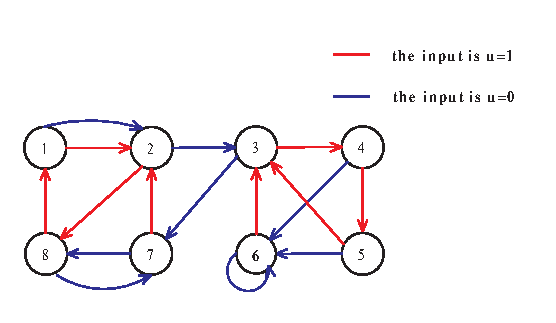
\includegraphics[width=3in]{state.eps}
\caption{The state transition graph}
\label{state}
\end{figure}
We can know that the BCN (\ref{ex1}) is controllable, since the state transition graph is strongly connected. But we can not find a state feedback controller which can make BCN (\ref{ex1}) be controllable. If there exist a state feedback controller, then for an arbitrary state $x\in \Delta_{8}$, there is only one control. So if BCN is controllable by a state feedback controller, then the state transition graph must be strongly connected, and the state transition graph like Fig. \ref{state1}.
\begin{figure}
\centering

\includegraphics[width=3in]{state1.eps}
\caption{The state transition graph with state feedback controller }
\label{state1}
\end{figure}
But in the state transition graph of BCN (\ref{ex1}), we can not find a subgraph which contains all states like Fig. \ref{state1}. Hence, there is not a state feedback controler such that BCN (\ref{ex1}) is controllable.
\end{example}


\section{EXAMPLE}
A brief example is given to depict the equivalence between free control sequence and  feedback controller.
\begin{example}
Consider the following Boolean control network with 3 states and a input:
\begin{eqnarray}\label{ex3}
 \left\{ \begin{aligned}
&x_1(t+1)=\neg u(t)\wedge(x_2(t)\vee x_3(t)),\\
&x_2(t+1)=\neg u(t)\wedge x_1(t),\\
&x_3(t+1)=u(t)\wedge x_1(t).
\end{aligned} \right.
\end{eqnarray}
By using Lemma \ref{lemma}, we can obtain the algebraic form of (\ref{ex3}):
\begin{equation}
x(t+1)=L_2u(t)x(t),
\end{equation}
where $L=[7~7~7~7~8~8~8~8~2~2~2~6~4~4~4~8]$. By using Algorithm 1, we can know that $K=2$, the BCN (\ref{ex3}) can be stabilized to state $\delta^8_{8}$ by free control sequence. Hence, we can use Algorithm 2, the state feedback controller is $u(t)=Fx(t)$ with $F=[1~1~1~1~1~1~1~1]$.
The state transition graph is shown as follows:
\begin{figure}
\centering
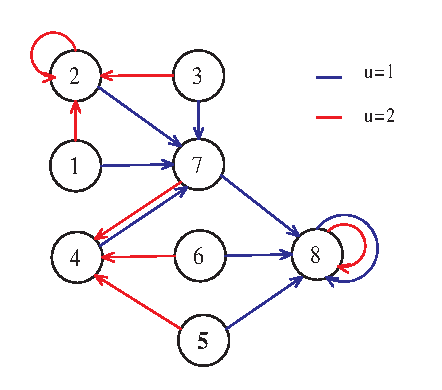
\includegraphics[width=2in]{ex2.eps}
\caption{The state transition graph in Example 2}
\label{ex2}
\end{figure}
\end{example}
From the state transition graph Fig. 2, we can know that BCN (\ref{ex3}) is stabilized to state $\delta^8_8$, which is coincident with our results.

%%%%%%%%%%%%%%%%%%%%%%%%%%%%%%%%%%%%%%%%%%%%%%%%%%%%%%%%%%%%%%%%%%%%%%%%%%%%%%%%
\section{CONCLUSION}
In this paper, by using the method of STP, we obtained the algebraic form of BCN. Based on the algebraic form of BCN, we investigated the effect of free control sequence and state feedback controller on the problem of stabilization of BCN. We obtain that the effect of these two controller is same on the problem of stabilization of BCN and provide two algorithms to obtain the state feedback controller. Then we prove that the effects of free control sequence and state feedback controller on the problem of global controllability are not same. Finally, an example is provide to illustrate the results we obtained.
%%%%%%%%%%%%%%%%%%%%%%%%%%%%%%%%%%%%%%%%%%%%%%%%%%%%%%%%%%%%%%%%%%%%%%%%%%%%%%%
%%%%%%%%%%%%%%%%%%%%%%%%%%%%%%%%%%%%%%%%%%%%%%%%%%%%%%%%%%%%%%%%%%%%%%%%%%%%%%%%
\bibliographystyle{ieeetr}
\bibliography{F:/FreeandFeedback/reference}

\end{document}
